\documentclass[twocolumn]{article}

\usepackage[]{animate}
\usepackage[]{graphicx}
\usepackage{hyperref}
\usepackage[]{cite}

\begin{document}

\title{The MacKay Effect}
\author{J. A. Kilgallen}
\maketitle

\begin{abstract}
The \emph{MacKay effect} is a visual aftereffect which is perceived following exposure to stimuli
consisting of spatially repetitive patterns. Presently there is no widely accepted explanation
of the effect in terms of the adaptation of neurons tuned to particular spatial orientations. 
Since it's discovery several variants of the effect have been discovered, some of which co-occur with
the better known \emph{motion aftereffect}. Relatively little is known about the effect when compared to other forms of 
visual illusion like contour completion or the tilt illusion. This review discusses the established knowledge of the effect
focusing primarily on the different variants of the stimulus and what this reveals about the mechanism which causes the effect.
\end{abstract}

\section[]{Introduction}
After prolonged adaptation to an image containing spatially repetitive patterns, 
observation of a homogenous background evokes the perception of an after image 
which is said to be approximately orthogonal to the original stimulus known as the emph{Complementary Image} (CI)\cite{mackay_1957a,mackay_1957b}. 
As is the case with many perceptual phenomena, the effect was originally described by Purkinje~\cite{wade_1977}.
Since then the effect has been rediscovered numerous times~\cite{wade_1977}, most famously by physicist D. M. Mackay~\cite{mackay_1957a}.

\section[]{Variants of the Effect}
There are two primary variations of the stimulus: static and dynamic. 
In the static variant of the stimulus the observer views a still image exhibiting repetitive
spatial patterns. While this variant of the stimulus is robust and can cause the perception of an after image
after only a few seconds, studies have shown that the effect does not occur under image stabilization~\cite{pritchard_1958}.

In the dynamic variant a stimulus with spatially repetitive patterns which flickers at a constant speed is viewed. 
The dynamic variant has been shown to demonstrate several other interesting properties. For instance, if the center or surround portion
of the image is homogenous, and flickers at the same rate as the rest of the image the CI can then extend to fill the rest of the visual field~\cite{billock_2007}.

Both the static and dynamic variants can occur with a variety of spatially repetitive patterns, with the most well researched being radial patterns, concentric circles, and squared sinusoidal gratings. 
These each evoke CIs of wavy lines which are approximately orthogonal to the stimulus. Examples of these stimuli are presented bellow as figures~\ref{fig:rays},~\ref{fig:circles} and~\ref{fig:gratings} respectively.
The embedded images are examples of the static variants, however the images also serve as links to the dynamic variants of the stimuli.

A new variant of the effect currently being explored is a randomly shaded version of the dynamic stimulus, in which each homogenous
component of the image is colored pseudorandomly to investigate if this has any effect on the strength of the CI perceived.

\section[]{Conclusion}
The MacKay effect is a significantly underresearched form of optical illusion, and exploration of its mechanism
could lead to significant improvements in our understanding of the organization of visual processing in the brain by 
providing evidence of pattern opponency. However, further research is required to develop any credible theories. 

\begin{figure}
    \begin{center}
        \caption[]{}%
        \label{fig:rays}
        \href{run:plots/ray_flicker_1024_1024_4_4_0.gif}{
\includegraphics[width=0.85\columnwidth]{plots/ray_static_1024_1024_4_4.png}}
    \end{center}
\end{figure}

\begin{figure}
    \begin{center}
        \caption[]{}%
        \label{fig:circles}
        \href{run:plots/circle_flicker_1024_1024_4_8_128.gif}{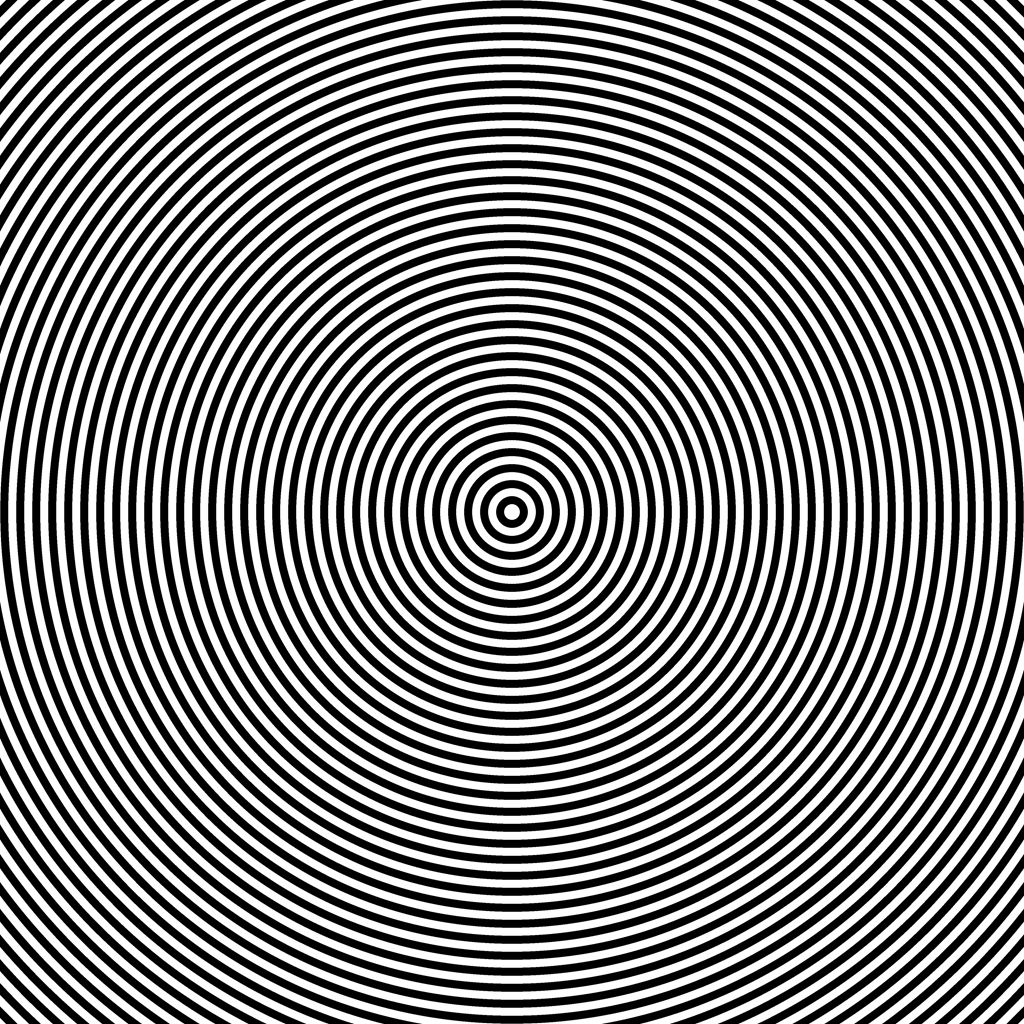
\includegraphics[width=0.85\columnwidth]{plots/circle_static_1024_1024_4_8.png}}
    \end{center}
\end{figure}

\begin{figure}
    \begin{center}
        \caption[]{}%
        \label{fig:gratings}
        \href{run:plots/gratings_flicker_1024_1024_4_16_128.gif}{
\includegraphics[width=0.85\columnwidth]{plots/gratings_static_1024_1024_4_16.png}}
    \end{center}
\end{figure}

\bibliographystyle{plain}
\bibliography{references}

\end{document}